\problemname{Neighborhood Watch}

Jennifer was nominated to be neighborhood watch captain and is now in charge of managing the watch for her street. 

Jennifer's street consists of houses on only one side of the road. She has a plan of which houses will be a \textit{neighborhood watch house} and wants to know how safe the plan is. A \textit{walk} from one house to another house (not necessarily distinct) is considered \textit{safe} if there is at least one house along the walk that is a neighborhood watch house. The \textit{safety rating} of a plan is the number of walks that are safe on the street. Since a walk is either safe or not safe, when traveling in either direction, it is not counted twice in the safety rating.

\begin{figure}[h]
\begin{center}
 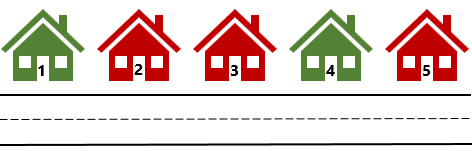
\includegraphics[width=0.7\textwidth]{houses}
 \caption{Sample input. One example of a safe walk is traveling from house $1$ to house $5$.
}
\end{center}
\end{figure}

Tell Jennifer the safety rating of her plan.

\section*{Input}

The first line of input contains two integers $N$~($1 \leq N \leq 200\,000$), which is the number of houses on the street, and $K$~($0 \leq K \leq N$), which is the number of neighborhood watch houses in Jennifer's plan. The houses are numbered $1, \dots , N$.

The next $K$ lines describe the neighborhood watch houses. Each of these lines contains a single integer $H$~($1 \leq H \leq N$), which is the house number of a neighborhood watch house. The house numbers are given in strictly increasing order.

\section*{Output}

Display the safety rating of Jennifer's plan.
